\documentclass[main.tex]{subfiles}

\begin{document}

% \textcolor{red}{Вводная лекция}

\section{Лекция 23.03.2021 (Донцов Е.В.)}

\subsection{Модель EP3D (Enhanced pdeudo-3D model)}

\includegraphics[width=\textwidth, page=73]{HF_slides.pdf}

\includegraphics[width=\textwidth, page=74]{HF_slides.pdf}

\includegraphics[width=\textwidth, page=75]{HF_slides.pdf}

\includegraphics[width=\textwidth, page=76]{HF_slides.pdf}

\includegraphics[width=\textwidth, page=77]{HF_slides.pdf}

\includegraphics[width=\textwidth, page=78]{HF_slides.pdf}

\includegraphics[width=\textwidth, page=79]{HF_slides.pdf}

\includegraphics[width=\textwidth, page=80]{HF_slides.pdf}

\includegraphics[width=\textwidth, page=81]{HF_slides.pdf}

\includegraphics[width=\textwidth, page=82]{HF_slides.pdf}

\includegraphics[width=\textwidth, page=83]{HF_slides.pdf}

\includegraphics[width=\textwidth, page=84]{HF_slides.pdf}

\includegraphics[width=\textwidth, page=85]{HF_slides.pdf}


\end{document}